\SourceLeaf{268}%
\noindent Auf der andern Seite ist für $dA = 0$ nach III.:
\[
\sin B \,.\, da = \cos B\, g(a) \,.\, db,
\]
also
\[
g(c) \sin A = g(a) \cos B,
\]
oder mit Hilfe von V. 2):
\[
\tag*{V. 3)} g(c) = g(a)\, g(b).
\]
Ferner ergibt sich aus V. 1) und V. 2) durch Multiplication:
\[
\mathrm{tg}\, A \,.\, \mathrm{tg}\, B \,.\, g(a)\, g(b) = 1,
\]
\Needspace{7\baselineskip}
was vermöge V. 3) in
\[
\tag*{V. 4)} \mathrm{tg}\, A \,.\, \mathrm{tg}\, B \,.\, g(c) = 1
\]
übergeht.

Man erkennt leicht, dass die Relationen V. 1), 2) und 3) ausreichen, um sämmtliche
10 Gleichungen herzuleiten, die zwischen je drei Stücken eines rechtwinkligen
Dreiecks bestehen, nemlich der Reihe nach zwischen
\[
\begin{array}{ll}
a,\ b,\ c & A,\ a,\ c;\ B,\ b,\ c\\
A,\ b,\ c;\ B,\ a,\ c & A,\ B,\ a;\ A,\ B,\ b\\
A,\ a,\ b;\ B,\ a,\ b & A,\ B,\ c.
\end{array}
\]
Es wird also alles darauf ankommen, die in diesen Relationen auftretende noch
unbekannte Function $g(x)$ zu bestimmen, wozu man mittelst folgender Überlegungen
gelangt.

12. In dem Dreieck $PQR$ sei der Winkel bei $Q$ ein Rechter, der Winkel bei $P$
unendlich klein, sodass sein Sinus durch den Bogen ersetzt werden kann. Dann
unterscheidet sich der Winkel bei $R$ unendlich wenig von einem Rechten, und die
Relation V. 1), in der man $A$, $B$ durch $R$, $P$ zu ersetzen hat, geht über in
\[
90^{0} - R = g(PQ) \,.\, P
\]
oder
\[
\tag*{(C)} R = 90^{0} - g(PQ) \,.\, P.
\]

\begin{center}\begin{minipage}{\linewidth}\centering
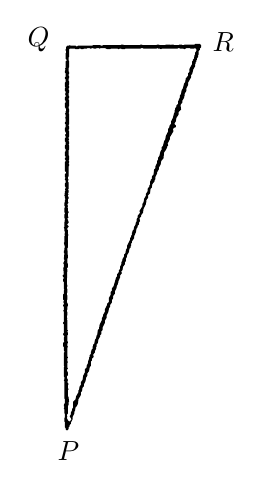
\begin{tikzpicture}[x=0.00744417cm,y=-0.00744417cm]
\fill[even odd rule] (315,50) -- (307,50) -- (306,51) -- (289,51) -- (288,52) -- (285,52) -- (284,51) -- (280,51) -- (279,52) -- (271,52) -- (270,51) -- (267,51) -- (266,52) -- (264,51) -- (257,51) -- (256,52) -- (246,52) -- (245,51) -- (242,51) -- (241,52) -- (217,52) -- (216,51) -- (214,51) -- (213,52) -- (185,52) -- (184,51) -- (181,51) -- (180,52) -- (150,52) -- (149,53) -- (146,53) -- (145,52) -- (133,52) -- (132,53) -- (107,53) -- (106,54) -- (104,54) -- (103,53) -- (95,53) -- (93,52) -- (92,53) -- (89,53) -- (87,55) -- (87,58) -- (86,59) -- (86,61) -- (87,62) -- (87,65) -- (86,66) -- (86,75) -- (88,77) -- (88,78) -- (86,80) -- (86,91) -- (85,92) -- (86,94) -- (85,96) -- (85,99) -- (86,100) -- (86,106) -- (85,107) -- (85,109) -- (86,110) -- (86,115) -- (85,116) -- (85,123) -- (86,124) -- (85,126) -- (85,130) -- (86,131) -- (86,134) -- (85,135) -- (86,137) -- (86,140) -- (85,141) -- (85,146) -- (86,147) -- (86,150) -- (85,151) -- (85,158) -- (87,161) -- (87,164) -- (86,165) -- (86,168) -- (85,169) -- (86,171) -- (86,175) -- (85,176) -- (86,177) -- (86,183) -- (85,184) -- (85,186) -- (86,187) -- (86,192) -- (85,193) -- (85,198) -- (87,203) -- (85,205) -- (86,207) -- (86,210) -- (85,211) -- (85,216) -- (86,217) -- (86,222) -- (85,223) -- (85,228) -- (86,229) -- (86,233) -- (85,234) -- (85,241) -- (86,242) -- (86,244) -- (85,245) -- (85,247) -- (86,248) -- (86,250) -- (85,251) -- (85,267) -- (87,269) -- (87,270) -- (85,272) -- (85,277) -- (86,278) -- (85,280) -- (85,282) -- (86,283) -- (86,287) -- (85,288) -- (85,293) -- (86,294) -- (86,296) -- (85,298) -- (86,300) -- (85,301) -- (84,309) -- (85,310) -- (85,313) -- (86,315) -- (85,316) -- (85,320) -- (84,321) -- (84,326) -- (85,327) -- (85,329) -- (84,330) -- (84,337) -- (85,338) -- (85,340) -- (84,341) -- (84,347) -- (85,348) -- (85,351) -- (84,352) -- (85,353) -- (84,354) -- (84,362) -- (83,363) -- (84,365) -- (84,369) -- (85,370) -- (85,373) -- (84,374) -- (85,376) -- (84,378) -- (84,388) -- (83,389) -- (85,397) -- (84,398) -- (84,402) -- (83,403) -- (83,406) -- (84,407) -- (83,417) -- (84,418) -- (84,420) -- (82,424) -- (83,426) -- (83,431) -- (82,432) -- (83,443) -- (81,445) -- (81,446) -- (83,449) -- (82,451) -- (82,455) -- (83,456) -- (83,468) -- (84,469) -- (83,471) -- (83,476) -- (82,477) -- (82,486) -- (83,487) -- (83,489) -- (82,490) -- (83,492) -- (83,494) -- (82,495) -- (82,497) -- (83,498) -- (83,504) -- (82,505) -- (83,507) -- (83,524) -- (82,525) -- (82,527) -- (83,528) -- (83,543) -- (82,544) -- (82,546) -- (84,549) -- (83,551) -- (83,555) -- (84,557) -- (82,560) -- (82,566) -- (83,567) -- (83,573) -- (84,574) -- (84,576) -- (83,577) -- (83,599) -- (84,600) -- (83,602) -- (83,617) -- (84,618) -- (84,622) -- (83,624) -- (84,625) -- (84,655) -- (85,656) -- (85,662) -- (83,666) -- (83,668) -- (84,669) -- (83,672) -- (84,673) -- (84,680) -- (85,681) -- (85,687) -- (84,688) -- (84,694) -- (85,695) -- (85,704) -- (86,705) -- (86,707) -- (88,709) -- (89,709) -- (91,707) -- (91,704) -- (93,702) -- (93,700) -- (95,698) -- (95,696) -- (98,690) -- (98,686) -- (101,680) -- (101,677) -- (102,676) -- (103,670) -- (105,668) -- (107,664) -- (108,656) -- (112,649) -- (112,644) -- (114,642) -- (115,636) -- (117,634) -- (117,631) -- (120,625) -- (121,619) -- (123,616) -- (123,612) -- (126,608) -- (127,602) -- (129,599) -- (129,592) -- (131,590) -- (131,587) -- (134,584) -- (133,580) -- (136,576) -- (136,574) -- (138,570) -- (138,567) -- (139,566) -- (139,562) -- (141,560) -- (142,554) -- (145,549) -- (145,547) -- (147,545) -- (147,540) -- (149,538) -- (149,534) -- (153,526) -- (153,522) -- (156,517) -- (156,513) -- (159,507) -- (160,501) -- (162,498) -- (162,495) -- (165,491) -- (165,487) -- (167,484) -- (167,480) -- (170,476) -- (170,472) -- (173,466) -- (173,464) -- (174,463) -- (174,461) -- (175,460) -- (175,458) -- (176,457) -- (176,455) -- (179,448) -- (179,445) -- (182,441) -- (181,438) -- (183,436) -- (184,430) -- (187,426) -- (187,423) -- (189,420) -- (189,416) -- (190,415) -- (191,410) -- (194,405) -- (195,399) -- (197,397) -- (197,395) -- (198,394) -- (198,390) -- (199,389) -- (199,387) -- (203,381) -- (203,378) -- (206,371) -- (207,365) -- (209,362) -- (209,360) -- (211,358) -- (211,355) -- (213,352) -- (212,347) -- (215,344) -- (215,342) -- (218,338) -- (219,331) -- (223,323) -- (223,321) -- (224,320) -- (224,316) -- (227,312) -- (227,308) -- (230,305) -- (231,297) -- (233,295) -- (234,289) -- (238,284) -- (238,282) -- (239,281) -- (239,277) -- (242,271) -- (242,269) -- (245,264) -- (245,261) -- (248,256) -- (249,250) -- (253,245) -- (254,235) -- (257,231) -- (259,227) -- (259,225) -- (261,223) -- (260,220) -- (264,212) -- (264,209) -- (270,199) -- (269,195) -- (271,193) -- (274,192) -- (274,189) -- (272,187) -- (272,185) -- (274,182) -- (275,176) -- (279,170) -- (279,166) -- (283,162) -- (282,154) -- (285,150) -- (285,147) -- (288,142) -- (288,140) -- (289,139) -- (289,135) -- (292,130) -- (292,126) -- (295,120) -- (295,116) -- (300,107) -- (300,103) -- (302,101) -- (304,93) -- (307,88) -- (307,84) -- (308,83) -- (308,81) -- (309,80) -- (309,78) -- (310,77) -- (310,75) -- (312,72) -- (312,69) -- (313,68) -- (313,62) -- (315,60) -- (315,58) -- (317,56) -- (317,52) -- cycle
(307,57) -- (309,59) -- (309,62) -- (307,65) -- (307,68) -- (306,69) -- (305,75) -- (303,77) -- (303,79) -- (302,80) -- (302,84) -- (297,93) -- (297,98) -- (295,100) -- (295,104) -- (291,109) -- (290,115) -- (288,118) -- (286,126) -- (284,129) -- (283,135) -- (281,138) -- (281,141) -- (278,148) -- (278,152) -- (275,155) -- (275,157) -- (273,160) -- (273,162) -- (272,163) -- (272,167) -- (271,168) -- (269,176) -- (266,182) -- (266,186) -- (263,190) -- (263,192) -- (261,195) -- (261,199) -- (257,207) -- (256,213) -- (254,216) -- (252,224) -- (250,226) -- (250,230) -- (248,233) -- (246,241) -- (244,244) -- (244,247) -- (242,250) -- (242,253) -- (239,259) -- (239,262) -- (237,264) -- (236,273) -- (234,275) -- (233,277) -- (233,280) -- (231,282) -- (231,284) -- (230,285) -- (230,290) -- (229,291) -- (229,293) -- (226,297) -- (226,301) -- (223,306) -- (223,309) -- (220,314) -- (219,320) -- (217,323) -- (217,327) -- (212,335) -- (213,338) -- (209,343) -- (209,346) -- (207,349) -- (207,353) -- (206,354) -- (205,359) -- (203,362) -- (202,367) -- (200,369) -- (200,371) -- (199,372) -- (199,376) -- (198,377) -- (198,379) -- (196,381) -- (196,384) -- (191,394) -- (191,398) -- (189,401) -- (188,407) -- (186,409) -- (186,412) -- (183,417) -- (183,419) -- (181,423) -- (181,426) -- (179,430) -- (179,434) -- (177,436) -- (177,439) -- (174,443) -- (174,446) -- (172,449) -- (168,463) -- (165,467) -- (165,471) -- (163,473) -- (163,478) -- (160,483) -- (160,490) -- (157,493) -- (157,495) -- (153,503) -- (153,507) -- (150,512) -- (150,514) -- (148,518) -- (148,521) -- (144,529) -- (143,536) -- (141,538) -- (140,546) -- (139,547) -- (138,552) -- (136,555) -- (135,561) -- (133,563) -- (133,565) -- (132,566) -- (132,570) -- (130,572) -- (130,574) -- (129,575) -- (129,579) -- (127,581) -- (127,584) -- (126,585) -- (126,588) -- (125,589) -- (124,595) -- (122,599) -- (122,602) -- (119,605) -- (119,610) -- (116,616) -- (115,623) -- (112,627) -- (112,632) -- (110,634) -- (109,640) -- (108,641) -- (108,644) -- (104,651) -- (103,656) -- (99,660) -- (99,670) -- (97,673) -- (97,675) -- (95,679) -- (95,682) -- (93,685) -- (96,690) -- (95,692) -- (93,694) -- (92,694) -- (90,692) -- (88,688) -- (89,686) -- (88,683) -- (90,680) -- (90,667) -- (91,666) -- (91,661) -- (92,660) -- (91,652) -- (90,651) -- (90,640) -- (91,639) -- (90,637) -- (90,632) -- (91,630) -- (89,627) -- (90,623) -- (88,619) -- (88,617) -- (90,615) -- (90,611) -- (88,606) -- (90,604) -- (89,602) -- (89,594) -- (90,593) -- (89,591) -- (89,586) -- (90,585) -- (89,583) -- (89,568) -- (90,567) -- (89,565) -- (89,561) -- (90,560) -- (90,558) -- (89,557) -- (89,547) -- (90,546) -- (90,543) -- (89,541) -- (90,539) -- (89,538) -- (89,521) -- (88,520) -- (89,518) -- (88,516) -- (88,514) -- (89,513) -- (89,507) -- (88,506) -- (88,504) -- (89,503) -- (89,498) -- (90,497) -- (90,494) -- (88,490) -- (88,487) -- (89,486) -- (89,479) -- (88,478) -- (88,475) -- (89,474) -- (89,468) -- (88,467) -- (88,465) -- (89,464) -- (89,461) -- (88,460) -- (89,435) -- (88,433) -- (90,431) -- (90,425) -- (89,424) -- (89,416) -- (90,415) -- (89,398) -- (90,397) -- (90,377) -- (91,376) -- (90,374) -- (90,368) -- (89,367) -- (89,364) -- (91,362) -- (91,361) -- (89,359) -- (89,357) -- (91,355) -- (91,353) -- (89,348) -- (91,346) -- (90,344) -- (90,339) -- (91,338) -- (91,336) -- (90,335) -- (90,330) -- (89,329) -- (90,327) -- (89,323) -- (91,321) -- (90,319) -- (90,315) -- (91,314) -- (91,311) -- (90,310) -- (90,308) -- (91,307) -- (90,305) -- (91,303) -- (91,300) -- (90,299) -- (91,297) -- (91,286) -- (90,285) -- (91,281) -- (90,280) -- (90,277) -- (91,276) -- (91,259) -- (92,258) -- (92,255) -- (91,254) -- (92,252) -- (92,250) -- (91,249) -- (92,247) -- (92,241) -- (91,240) -- (91,231) -- (92,230) -- (92,223) -- (91,222) -- (92,220) -- (92,217) -- (91,216) -- (91,214) -- (92,213) -- (91,211) -- (91,209) -- (92,208) -- (92,199) -- (91,198) -- (91,196) -- (92,195) -- (92,191) -- (91,190) -- (91,188) -- (92,187) -- (92,169) -- (91,168) -- (92,166) -- (92,161) -- (91,160) -- (91,157) -- (92,156) -- (92,146) -- (91,145) -- (91,143) -- (92,142) -- (92,139) -- (91,138) -- (91,134) -- (92,133) -- (92,129) -- (91,128) -- (91,126) -- (92,125) -- (92,122) -- (91,121) -- (92,119) -- (92,114) -- (91,113) -- (91,109) -- (92,108) -- (92,105) -- (91,104) -- (91,102) -- (92,101) -- (92,98) -- (91,97) -- (91,91) -- (92,90) -- (92,79) -- (91,78) -- (91,73) -- (92,72) -- (92,59) -- (93,58) -- (102,58) -- (103,59) -- (108,59) -- (109,58) -- (112,58) -- (113,59) -- (116,59) -- (117,58) -- (122,58) -- (123,57) -- (127,57) -- (128,58) -- (130,58) -- (131,57) -- (133,57) -- (134,58) -- (138,58) -- (139,57) -- (143,57) -- (144,58) -- (146,57) -- (153,57) -- (157,59) -- (162,59) -- (163,58) -- (175,58) -- (176,59) -- (178,58) -- (181,58) -- (182,59) -- (187,59) -- (188,58) -- (214,58) -- (215,57) -- (218,57) -- (219,58) -- (241,58) -- (243,57) -- (244,58) -- (247,58) -- (249,59) -- (250,58) -- (277,58) -- (278,57) -- (280,57) -- (281,58) -- (287,58) -- (289,59) -- (292,57) -- (298,57) -- (299,58) -- (305,58) -- cycle;
\node[inner sep=0pt,font=\fontsize{10}{12}\selectfont] at (40,43) {$Q$};
\node[inner sep=0pt,font=\fontsize{10}{12}\selectfont] at (355,46) {$R$};
\node[inner sep=0pt,font=\fontsize{10}{12}\selectfont] at (91,744) {$P$};
\end{tikzpicture}


Fig. 9.
\end{minipage}\end{center}

13. Das Viereck $PQRS$ habe in $P$, $Q$ und $R$ rechte Winkel, während die Seite
$PQ$ unendlich klein ist. Die Diagonale $QS$ sei gleich $r$. Dann hat man nach
(A'):
\[
PQ = f(r) \,.\, PSQ
\]
oder
\[
PSQ = \frac{PQ}{f(r)},
\]
und ebenso ist
\[
RQS = \frac{RS}{f(r)}.
\]
Verlängert man jetzt $PQ$ um $QT = PQ$, $SR$ um $RU = SR$, so hat das Viereck
$PTUS$ in $P$ und $T$ rechte Winkel, und die Seiten $PS$ und $TU$ sind einander
gleich. Mithin ist nach (B):
\[
SU = g(PS) \,.\, PT
\]
oder, da $RS$ unendlich klein ist, bis auf unendlich kleine Grössen zweiter
Ordnung:
\[
RS = g(r) \,.\, PQ
\]
und mit derselben Genauigkeit:
\[
\tag*{7)} RQS = \frac{g(r)}{f(r)} \,.\, PQ.
\]

\begin{center}\begin{minipage}{\linewidth}\centering
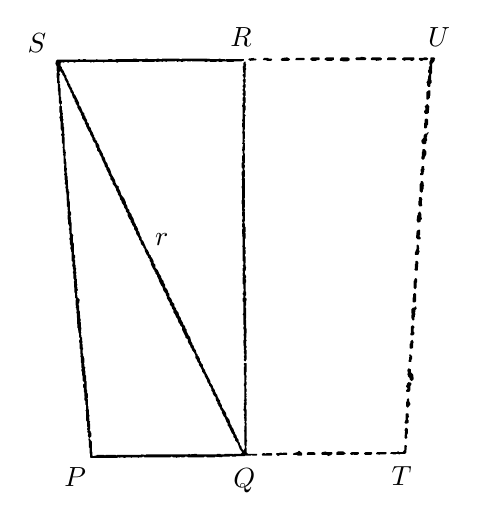
\begin{tikzpicture}[x=0.00733591cm,y=-0.00733591cm]
\fill[even odd rule] (423,755) -- (424,757) -- (440,757) -- (441,756) -- (441,754) -- (440,753) -- (431,753) -- (430,754) -- (428,753) -- (425,753) -- cycle
(448,754) -- (448,755) -- (451,758) -- (455,756) -- (466,756) -- (467,755) -- (467,753) -- (466,752) -- (460,752) -- (459,753) -- (457,752) -- (454,752) -- (453,753) -- (449,753) -- cycle
(621,754) -- (622,755) -- (625,755) -- (626,756) -- (627,755) -- (637,755) -- (639,753) -- (639,752) -- (638,751) -- (623,751) -- (621,753) -- cycle
(600,753) -- (600,754) -- (602,756) -- (612,756) -- (614,754) -- (614,752) -- (613,751) -- (603,751) -- cycle
(576,753) -- (576,754) -- (578,756) -- (580,756) -- (581,755) -- (583,756) -- (588,756) -- (591,754) -- (591,752) -- (590,751) -- (579,751) -- cycle
(501,753) -- (501,755) -- (502,756) -- (515,756) -- (516,755) -- (516,753) -- (513,751) -- (503,751) -- cycle
(552,752) -- (552,755) -- (553,756) -- (564,756) -- (568,754) -- (568,753) -- (564,750) -- (555,750) -- cycle
(526,753) -- (526,754) -- (528,756) -- (536,756) -- (538,758) -- (543,756) -- (545,754) -- (545,752) -- (544,751) -- (535,751) -- (534,750) -- (528,751) -- cycle
(493,753) -- (488,749) -- (487,749) -- (485,751) -- (478,753) -- (477,755) -- (478,756) -- (484,756) -- (485,757) -- (492,757) -- (493,756) -- cycle
(674,741) -- (673,739) -- (671,739) -- (670,740) -- (670,747) -- (667,751) -- (661,751) -- (660,750) -- (658,750) -- (657,751) -- (647,751) -- (645,753) -- (646,754) -- (649,754) -- (650,755) -- (655,755) -- (656,754) -- (659,754) -- (660,755) -- (662,755) -- (663,754) -- (671,754) -- (673,752) -- cycle
(674,709) -- (672,709) -- (670,713) -- (671,715) -- (670,726) -- (672,728) -- (673,728) -- (675,726) -- (674,722) -- (676,718) -- (676,712) -- cycle
(676,684) -- (673,684) -- (672,685) -- (672,695) -- (670,700) -- (672,702) -- (674,702) -- (677,700) -- (677,696) -- (676,695) -- (676,693) -- (678,689) -- (677,688) -- (677,685) -- cycle
(677,658) -- (676,658) -- (674,660) -- (674,663) -- (673,664) -- (673,672) -- (675,674) -- (676,674) -- (680,669) -- (680,667) -- (678,663) -- (678,659) -- cycle
(681,631) -- (677,630) -- (674,633) -- (674,635) -- (673,636) -- (673,638) -- (675,640) -- (675,642) -- (673,644) -- (673,646) -- (674,647) -- (678,647) -- (680,644) -- (680,637) -- (682,634) -- (682,632) -- cycle
(677,606) -- (675,609) -- (675,611) -- (676,612) -- (675,617) -- (676,618) -- (676,620) -- (679,623) -- (679,625) -- (682,628) -- (683,628) -- (686,625) -- (685,617) -- (681,613) -- (681,608) -- cycle
(679,582) -- (678,583) -- (679,586) -- (678,587) -- (678,591) -- (677,592) -- (677,594) -- (678,595) -- (681,595) -- (682,594) -- (682,591) -- (683,590) -- (683,585) -- (680,582) -- cycle
(684,557) -- (683,557) -- (680,560) -- (680,563) -- (679,564) -- (679,571) -- (680,572) -- (683,572) -- (685,570) -- (685,563) -- (686,561) -- cycle
(685,532) -- (683,532) -- (681,534) -- (681,545) -- (680,546) -- (680,548) -- (681,549) -- (685,549) -- (687,547) -- (687,544) -- (686,543) -- (686,537) -- (687,536) -- (687,534) -- cycle
(690,499) -- (689,499) -- (687,501) -- (685,501) -- (682,504) -- (682,511) -- (683,512) -- (682,514) -- (682,519) -- (684,523) -- (686,523) -- (687,522) -- (687,518) -- (688,517) -- (688,514) -- (689,513) -- (688,509) -- (689,508) -- (689,505) -- (691,503) -- cycle
(688,476) -- (687,476) -- (685,478) -- (685,483) -- (684,484) -- (684,491) -- (685,492) -- (688,492) -- (690,490) -- (690,478) -- cycle
(690,450) -- (689,450) -- (687,452) -- (687,454) -- (686,455) -- (686,467) -- (688,469) -- (689,469) -- (691,466) -- (691,458) -- (692,457) -- (692,452) -- cycle
(690,420) -- (689,421) -- (689,425) -- (688,426) -- (688,433) -- (687,435) -- (689,437) -- (692,437) -- (693,436) -- (694,423) -- (692,420) -- cycle
(693,392) -- (691,393) -- (691,399) -- (688,406) -- (688,409) -- (689,410) -- (693,410) -- (695,408) -- (695,406) -- (696,405) -- (696,403) -- (695,402) -- (695,399) -- (696,398) -- (695,397) -- (695,394) -- cycle
(696,366) -- (693,367) -- (691,369) -- (690,380) -- (693,383) -- (697,383) -- (698,382) -- (698,380) -- (696,378) -- (696,376) -- (697,375) -- (697,367) -- cycle
(697,335) -- (696,335) -- (693,338) -- (693,341) -- (692,342) -- (691,350) -- (693,354) -- (697,353) -- (698,352) -- (698,350) -- (700,348) -- (700,346) -- (699,345) -- (699,339) -- cycle
(696,310) -- (695,311) -- (695,316) -- (694,317) -- (694,323) -- (696,326) -- (699,326) -- (701,324) -- (700,322) -- (700,316) -- (701,314) -- (699,310) -- cycle
(701,282) -- (699,282) -- (698,283) -- (698,285) -- (696,288) -- (696,299) -- (699,302) -- (700,302) -- (702,300) -- (702,297) -- (703,296) -- (703,291) -- (704,290) -- (703,288) -- (703,285) -- cycle
(703,256) -- (701,256) -- (699,258) -- (699,261) -- (698,262) -- (698,265) -- (699,267) -- (697,269) -- (697,271) -- (698,272) -- (701,272) -- (703,270) -- (703,267) -- (704,266) -- (704,263) -- (705,262) -- (704,260) -- (704,257) -- cycle
(705,227) -- (702,227) -- (701,228) -- (701,231) -- (700,232) -- (700,239) -- (699,240) -- (699,243) -- (701,245) -- (703,245) -- (705,243) -- (705,241) -- (708,235) -- (708,231) -- cycle
(712,198) -- (710,198) -- (708,200) -- (706,200) -- (704,202) -- (703,204) -- (703,207) -- (699,212) -- (700,216) -- (702,218) -- (706,218) -- (708,216) -- (708,213) -- (709,212) -- (709,209) -- (708,207) -- (709,206) -- (709,203) -- cycle
(709,174) -- (707,174) -- (705,176) -- (705,181) -- (704,182) -- (704,190) -- (705,191) -- (707,191) -- (709,189) -- (709,186) -- (711,184) -- (711,176) -- cycle
(710,149) -- (709,149) -- (705,153) -- (706,155) -- (706,159) -- (704,161) -- (704,163) -- (706,166) -- (709,166) -- (712,164) -- (713,153) -- cycle
(714,125) -- (712,125) -- (708,128) -- (708,140) -- (709,141) -- (711,141) -- (714,138) -- (714,135) -- (715,134) -- (715,126) -- cycle
(394,75) -- (391,78) -- (391,83) -- (390,84) -- (391,94) -- (392,95) -- (392,96) -- (390,98) -- (390,100) -- (391,101) -- (392,105) -- (390,108) -- (391,110) -- (391,116) -- (390,117) -- (390,119) -- (391,120) -- (391,122) -- (390,123) -- (390,126) -- (391,127) -- (391,129) -- (390,130) -- (390,133) -- (391,134) -- (391,137) -- (390,138) -- (390,143) -- (391,144) -- (391,146) -- (390,147) -- (390,150) -- (389,151) -- (389,153) -- (390,154) -- (390,175) -- (389,176) -- (389,178) -- (390,179) -- (390,181) -- (389,182) -- (389,188) -- (390,189) -- (390,196) -- (389,197) -- (390,198) -- (389,199) -- (390,200) -- (390,215) -- (389,217) -- (391,219) -- (391,220) -- (390,221) -- (389,229) -- (390,230) -- (390,234) -- (391,236) -- (389,239) -- (389,247) -- (390,249) -- (388,251) -- (388,258) -- (390,261) -- (390,264) -- (388,267) -- (388,272) -- (389,273) -- (389,278) -- (388,279) -- (389,281) -- (389,290) -- (388,291) -- (388,294) -- (389,295) -- (389,315) -- (388,316) -- (388,321) -- (389,322) -- (389,333) -- (390,334) -- (389,336) -- (389,342) -- (390,343) -- (390,348) -- (389,349) -- (389,352) -- (390,353) -- (390,355) -- (389,356) -- (389,361) -- (390,362) -- (390,365) -- (389,366) -- (389,374) -- (390,375) -- (389,377) -- (390,379) -- (390,393) -- (389,395) -- (390,396) -- (390,420) -- (391,421) -- (391,427) -- (390,428) -- (391,430) -- (391,432) -- (390,433) -- (390,438) -- (391,439) -- (390,441) -- (390,446) -- (391,447) -- (390,449) -- (390,460) -- (391,461) -- (391,468) -- (392,469) -- (391,475) -- (390,476) -- (390,478) -- (391,479) -- (391,484) -- (390,485) -- (390,490) -- (391,491) -- (391,511) -- (390,513) -- (391,514) -- (391,530) -- (392,531) -- (392,534) -- (391,535) -- (391,538) -- (392,539) -- (392,547) -- (391,548) -- (392,550) -- (392,557) -- (391,558) -- (391,562) -- (392,564) -- (391,566) -- (392,567) -- (392,574) -- (393,575) -- (392,577) -- (392,580) -- (393,581) -- (393,584) -- (392,585) -- (393,589) -- (392,590) -- (392,592) -- (394,594) -- (395,594) -- (397,590) -- (397,584) -- (396,583) -- (397,581) -- (397,575) -- (396,574) -- (396,571) -- (397,570) -- (397,568) -- (396,567) -- (396,559) -- (397,558) -- (396,556) -- (397,538) -- (396,537) -- (396,522) -- (395,521) -- (396,519) -- (396,502) -- (395,501) -- (395,498) -- (396,497) -- (396,489) -- (397,488) -- (397,486) -- (394,483) -- (396,479) -- (396,474) -- (395,473) -- (395,458) -- (396,457) -- (396,453) -- (395,452) -- (395,450) -- (396,449) -- (396,447) -- (394,443) -- (394,438) -- (395,437) -- (396,431) -- (395,430) -- (395,427) -- (394,426) -- (395,424) -- (395,413) -- (394,412) -- (394,409) -- (395,408) -- (395,402) -- (394,401) -- (395,399) -- (395,397) -- (394,396) -- (394,382) -- (395,381) -- (395,373) -- (394,371) -- (395,370) -- (395,362) -- (394,361) -- (394,356) -- (393,355) -- (393,352) -- (394,351) -- (394,336) -- (393,335) -- (394,333) -- (394,331) -- (393,330) -- (393,328) -- (394,327) -- (394,315) -- (393,314) -- (393,312) -- (394,311) -- (394,278) -- (393,277) -- (393,275) -- (394,274) -- (394,264) -- (393,263) -- (393,259) -- (394,258) -- (394,255) -- (393,254) -- (393,251) -- (394,250) -- (394,235) -- (393,234) -- (393,229) -- (394,228) -- (394,217) -- (393,216) -- (393,214) -- (394,213) -- (393,211) -- (393,209) -- (394,208) -- (394,197) -- (393,196) -- (393,193) -- (394,192) -- (394,170) -- (395,169) -- (395,168) -- (393,166) -- (393,164) -- (394,163) -- (394,160) -- (395,159) -- (395,152) -- (394,151) -- (394,147) -- (395,146) -- (395,138) -- (394,137) -- (394,135) -- (395,134) -- (395,126) -- (394,125) -- (394,121) -- (395,120) -- (395,115) -- (394,114) -- (394,112) -- (395,111) -- (395,106) -- (394,105) -- (394,103) -- (395,102) -- (395,90) -- (396,89) -- (396,87) -- (395,86) -- (396,80) -- (395,79) -- (395,76) -- cycle
(69,72) -- (67,74) -- (66,79) -- (68,83) -- (68,91) -- (69,92) -- (69,94) -- (68,95) -- (68,103) -- (69,104) -- (69,112) -- (70,113) -- (70,126) -- (71,127) -- (71,133) -- (72,134) -- (72,146) -- (74,150) -- (74,152) -- (73,153) -- (73,163) -- (74,164) -- (74,170) -- (73,171) -- (73,173) -- (74,174) -- (74,178) -- (75,179) -- (75,192) -- (77,196) -- (77,200) -- (76,201) -- (76,203) -- (77,204) -- (77,215) -- (79,219) -- (79,222) -- (78,224) -- (79,225) -- (79,233) -- (80,234) -- (79,236) -- (80,238) -- (80,251) -- (82,254) -- (81,256) -- (81,265) -- (82,266) -- (81,271) -- (82,272) -- (82,280) -- (83,281) -- (82,287) -- (84,289) -- (83,294) -- (84,295) -- (84,301) -- (85,302) -- (86,326) -- (87,327) -- (87,332) -- (88,333) -- (87,335) -- (87,338) -- (88,339) -- (87,341) -- (87,348) -- (88,349) -- (88,356) -- (90,360) -- (90,364) -- (89,365) -- (90,367) -- (90,373) -- (91,374) -- (91,380) -- (90,381) -- (90,383) -- (91,384) -- (91,391) -- (93,395) -- (92,397) -- (92,400) -- (93,401) -- (93,404) -- (94,405) -- (94,420) -- (96,422) -- (95,429) -- (96,430) -- (96,434) -- (97,435) -- (97,438) -- (96,439) -- (96,441) -- (97,442) -- (97,450) -- (99,454) -- (98,456) -- (99,475) -- (100,476) -- (100,484) -- (102,486) -- (101,488) -- (101,497) -- (102,498) -- (101,501) -- (102,502) -- (102,505) -- (103,506) -- (102,510) -- (103,511) -- (104,536) -- (105,537) -- (106,545) -- (107,546) -- (107,552) -- (109,555) -- (107,558) -- (107,561) -- (108,562) -- (108,572) -- (109,573) -- (109,581) -- (110,582) -- (109,586) -- (110,587) -- (110,596) -- (111,597) -- (111,605) -- (112,606) -- (111,608) -- (111,611) -- (112,612) -- (112,618) -- (113,619) -- (113,627) -- (116,631) -- (116,632) -- (114,634) -- (114,639) -- (115,640) -- (115,647) -- (116,648) -- (116,654) -- (117,655) -- (116,656) -- (117,657) -- (116,658) -- (116,661) -- (118,663) -- (118,669) -- (119,670) -- (119,678) -- (118,679) -- (119,681) -- (119,696) -- (121,699) -- (121,707) -- (122,708) -- (121,710) -- (121,712) -- (122,713) -- (121,716) -- (123,719) -- (122,723) -- (124,726) -- (123,730) -- (124,731) -- (124,743) -- (125,744) -- (125,753) -- (126,754) -- (126,760) -- (127,761) -- (173,761) -- (174,760) -- (176,760) -- (177,761) -- (179,760) -- (183,760) -- (184,761) -- (187,761) -- (188,760) -- (196,760) -- (197,761) -- (199,760) -- (208,760) -- (210,761) -- (211,760) -- (216,760) -- (217,759) -- (219,759) -- (220,760) -- (265,760) -- (266,759) -- (268,759) -- (269,760) -- (274,760) -- (276,761) -- (277,760) -- (281,760) -- (282,759) -- (284,760) -- (289,760) -- (290,759) -- (294,759) -- (295,760) -- (323,760) -- (324,759) -- (327,759) -- (328,760) -- (342,760) -- (343,759) -- (354,760) -- (355,759) -- (367,759) -- (368,758) -- (371,758) -- (372,759) -- (378,759) -- (379,758) -- (393,758) -- (394,757) -- (404,757) -- (405,756) -- (407,757) -- (414,757) -- (415,756) -- (415,754) -- (399,754) -- (397,752) -- (397,744) -- (396,743) -- (396,741) -- (397,740) -- (397,733) -- (398,732) -- (397,730) -- (397,726) -- (396,725) -- (397,724) -- (397,707) -- (396,706) -- (397,704) -- (397,701) -- (396,700) -- (396,698) -- (397,697) -- (397,692) -- (396,691) -- (397,690) -- (396,689) -- (397,688) -- (397,678) -- (396,677) -- (396,670) -- (397,669) -- (397,665) -- (396,664) -- (397,662) -- (397,659) -- (396,658) -- (396,656) -- (397,655) -- (396,653) -- (397,651) -- (396,649) -- (396,647) -- (397,646) -- (397,642) -- (396,641) -- (396,635) -- (397,634) -- (397,630) -- (396,629) -- (396,626) -- (397,625) -- (396,623) -- (397,621) -- (397,619) -- (396,618) -- (396,613) -- (397,612) -- (397,598) -- (396,597) -- (393,597) -- (392,598) -- (392,600) -- (393,601) -- (393,603) -- (392,604) -- (392,617) -- (393,618) -- (393,632) -- (392,633) -- (392,636) -- (393,637) -- (393,660) -- (392,662) -- (393,663) -- (393,665) -- (392,666) -- (392,669) -- (393,671) -- (392,672) -- (392,676) -- (391,678) -- (393,681) -- (393,685) -- (392,686) -- (393,690) -- (392,692) -- (393,693) -- (393,697) -- (394,698) -- (393,700) -- (394,705) -- (393,706) -- (393,713) -- (392,714) -- (393,716) -- (393,739) -- (394,740) -- (394,744) -- (392,748) -- (391,748) -- (388,744) -- (388,742) -- (385,738) -- (385,735) -- (383,733) -- (383,730) -- (380,726) -- (379,722) -- (377,720) -- (377,718) -- (375,715) -- (374,711) -- (371,707) -- (371,705) -- (369,703) -- (367,695) -- (362,689) -- (361,683) -- (354,673) -- (354,670) -- (351,665) -- (351,662) -- (349,660) -- (346,654) -- (346,652) -- (344,650) -- (342,646) -- (342,644) -- (339,640) -- (338,636) -- (334,631) -- (334,628) -- (325,611) -- (325,609) -- (323,607) -- (321,603) -- (321,600) -- (318,597) -- (318,595) -- (316,593) -- (316,590) -- (314,586) -- (312,584) -- (312,582) -- (310,580) -- (309,575) -- (306,571) -- (305,567) -- (303,565) -- (303,563) -- (301,560) -- (299,552) -- (297,550) -- (293,542) -- (293,539) -- (291,537) -- (290,533) -- (287,530) -- (287,528) -- (283,521) -- (283,519) -- (280,515) -- (279,510) -- (275,505) -- (275,503) -- (272,499) -- (272,495) -- (268,491) -- (268,489) -- (266,485) -- (263,482) -- (263,477) -- (261,475) -- (261,473) -- (259,469) -- (256,466) -- (256,462) -- (253,457) -- (253,455) -- (251,453) -- (249,449) -- (249,447) -- (246,443) -- (243,436) -- (239,432) -- (239,427) -- (236,424) -- (236,421) -- (233,415) -- (231,413) -- (231,411) -- (228,408) -- (228,406) -- (226,402) -- (224,400) -- (218,386) -- (215,383) -- (215,380) -- (213,377) -- (211,370) -- (209,368) -- (209,365) -- (207,361) -- (205,359) -- (205,357) -- (203,354) -- (201,347) -- (198,342) -- (198,340) -- (194,335) -- (194,332) -- (191,329) -- (190,324) -- (188,322) -- (188,319) -- (185,312) -- (180,306) -- (178,299) -- (175,294) -- (176,292) -- (172,289) -- (170,285) -- (169,280) -- (163,270) -- (161,263) -- (159,259) -- (157,257) -- (156,252) -- (153,248) -- (151,241) -- (149,239) -- (148,235) -- (142,224) -- (142,221) -- (140,217) -- (138,215) -- (138,213) -- (135,210) -- (135,208) -- (133,206) -- (133,203) -- (131,201) -- (131,199) -- (128,194) -- (127,190) -- (124,187) -- (124,183) -- (121,180) -- (121,177) -- (118,172) -- (118,170) -- (116,168) -- (116,165) -- (113,162) -- (110,154) -- (107,151) -- (107,147) -- (100,133) -- (98,131) -- (98,129) -- (95,124) -- (95,122) -- (92,118) -- (92,116) -- (89,112) -- (89,110) -- (85,103) -- (85,100) -- (83,98) -- (80,91) -- (77,87) -- (77,85) -- (75,83) -- (75,78) -- (77,76) -- (79,77) -- (81,77) -- (82,76) -- (86,76) -- (87,77) -- (89,77) -- (90,76) -- (97,76) -- (98,77) -- (100,77) -- (101,76) -- (126,76) -- (127,77) -- (129,76) -- (131,76) -- (132,77) -- (134,76) -- (148,76) -- (149,77) -- (151,76) -- (171,76) -- (172,77) -- (174,77) -- (175,76) -- (210,76) -- (211,75) -- (216,75) -- (217,76) -- (237,76) -- (238,75) -- (240,75) -- (241,76) -- (249,75) -- (251,76) -- (252,75) -- (256,75) -- (258,76) -- (259,75) -- (273,75) -- (274,74) -- (275,74) -- (277,76) -- (279,75) -- (283,75) -- (284,76) -- (286,76) -- (287,75) -- (290,75) -- (291,74) -- (293,74) -- (294,75) -- (300,75) -- (301,74) -- (303,75) -- (324,75) -- (325,76) -- (328,76) -- (329,75) -- (333,75) -- (334,76) -- (344,76) -- (345,75) -- (348,75) -- (349,76) -- (354,76) -- (355,75) -- (362,75) -- (363,76) -- (374,76) -- (375,75) -- (388,75) -- (389,74) -- (391,74) -- (392,73) -- (392,71) -- (362,71) -- (360,72) -- (359,71) -- (352,71) -- (351,70) -- (349,70) -- (348,71) -- (333,71) -- (332,70) -- (330,71) -- (328,70) -- (285,70) -- (284,71) -- (281,71) -- (280,70) -- (251,70) -- (250,71) -- (246,71) -- (245,70) -- (242,70) -- (241,71) -- (226,71) -- (225,70) -- (222,70) -- (221,71) -- (207,71) -- (206,70) -- (201,70) -- (200,71) -- (171,71) -- (170,72) -- (165,72) -- (164,71) -- (158,71) -- (157,72) -- (139,72) -- (138,71) -- (136,72) -- (119,72) -- (118,71) -- (114,71) -- (113,72) -- (109,72) -- (108,71) -- (106,71) -- (105,72) -- cycle
(74,92) -- (76,93) -- (76,94) -- (78,96) -- (78,98) -- (80,100) -- (82,104) -- (82,106) -- (86,113) -- (86,115) -- (92,126) -- (92,128) -- (94,130) -- (96,137) -- (99,141) -- (99,144) -- (101,146) -- (101,148) -- (104,152) -- (104,155) -- (110,165) -- (110,167) -- (112,170) -- (112,173) -- (117,180) -- (117,183) -- (119,185) -- (119,187) -- (123,195) -- (126,199) -- (126,201) -- (130,208) -- (130,210) -- (132,214) -- (135,217) -- (136,223) -- (138,225) -- (138,229) -- (142,233) -- (142,235) -- (146,242) -- (146,244) -- (151,254) -- (151,256) -- (154,260) -- (154,262) -- (158,269) -- (158,271) -- (161,275) -- (161,279) -- (164,282) -- (165,284) -- (165,287) -- (169,292) -- (171,296) -- (171,298) -- (174,303) -- (174,305) -- (177,309) -- (178,314) -- (180,316) -- (181,320) -- (184,324) -- (185,328) -- (188,332) -- (188,335) -- (191,338) -- (191,342) -- (194,348) -- (196,350) -- (196,353) -- (198,355) -- (199,358) -- (202,362) -- (202,365) -- (205,369) -- (206,374) -- (209,378) -- (211,382) -- (211,384) -- (213,386) -- (214,391) -- (218,395) -- (218,397) -- (220,399) -- (221,404) -- (224,410) -- (226,412) -- (226,414) -- (229,417) -- (229,420) -- (231,423) -- (231,426) -- (235,434) -- (237,436) -- (237,438) -- (239,440) -- (239,442) -- (242,445) -- (242,447) -- (245,453) -- (245,455) -- (249,463) -- (251,465) -- (253,472) -- (257,477) -- (257,479) -- (259,482) -- (259,485) -- (264,493) -- (264,496) -- (267,499) -- (268,503) -- (270,505) -- (270,509) -- (273,513) -- (275,518) -- (277,520) -- (279,527) -- (281,529) -- (282,532) -- (285,535) -- (285,539) -- (291,551) -- (291,553) -- (295,556) -- (295,560) -- (297,564) -- (299,566) -- (300,570) -- (302,572) -- (302,574) -- (306,579) -- (308,583) -- (308,588) -- (310,590) -- (312,595) -- (314,597) -- (314,600) -- (317,604) -- (320,610) -- (320,612) -- (324,617) -- (324,619) -- (328,626) -- (329,630) -- (332,634) -- (332,636) -- (334,638) -- (336,642) -- (336,645) -- (338,647) -- (338,649) -- (340,653) -- (343,656) -- (344,662) -- (346,664) -- (346,667) -- (348,669) -- (348,671) -- (350,673) -- (352,678) -- (354,680) -- (354,683) -- (357,689) -- (359,691) -- (362,699) -- (364,701) -- (364,705) -- (366,707) -- (371,718) -- (373,720) -- (374,722) -- (374,725) -- (377,728) -- (377,731) -- (381,735) -- (385,746) -- (389,751) -- (389,752) -- (387,754) -- (375,754) -- (374,755) -- (372,754) -- (359,754) -- (358,755) -- (352,755) -- (351,754) -- (346,754) -- (345,755) -- (311,755) -- (310,754) -- (299,755) -- (297,754) -- (296,755) -- (223,755) -- (222,756) -- (215,755) -- (214,756) -- (173,756) -- (172,757) -- (170,756) -- (153,756) -- (152,757) -- (150,756) -- (138,756) -- (137,757) -- (134,757) -- (133,758) -- (131,758) -- (130,757) -- (130,751) -- (129,750) -- (129,733) -- (125,728) -- (125,727) -- (128,724) -- (128,718) -- (127,717) -- (127,715) -- (125,713) -- (126,711) -- (126,702) -- (125,701) -- (126,698) -- (124,696) -- (125,694) -- (124,692) -- (125,687) -- (124,686) -- (124,678) -- (123,677) -- (123,672) -- (122,671) -- (122,660) -- (121,659) -- (122,657) -- (122,650) -- (121,649) -- (121,644) -- (120,643) -- (120,629) -- (119,628) -- (119,619) -- (118,618) -- (118,611) -- (117,610) -- (117,607) -- (118,605) -- (116,603) -- (116,599) -- (115,598) -- (116,596) -- (116,589) -- (115,588) -- (115,586) -- (114,585) -- (114,581) -- (113,580) -- (113,574) -- (114,573) -- (114,571) -- (113,570) -- (113,565) -- (112,564) -- (113,560) -- (112,559) -- (112,553) -- (111,552) -- (111,549) -- (110,548) -- (110,546) -- (111,545) -- (110,543) -- (111,536) -- (110,535) -- (110,527) -- (109,526) -- (110,522) -- (109,521) -- (108,507) -- (107,506) -- (107,498) -- (106,497) -- (106,494) -- (107,493) -- (108,487) -- (104,483) -- (104,480) -- (103,479) -- (103,477) -- (104,476) -- (103,473) -- (105,471) -- (105,470) -- (104,469) -- (104,466) -- (103,465) -- (104,461) -- (103,460) -- (103,452) -- (102,451) -- (102,445) -- (101,444) -- (102,442) -- (102,439) -- (101,438) -- (102,433) -- (101,432) -- (101,428) -- (100,427) -- (100,419) -- (99,418) -- (99,416) -- (100,415) -- (100,411) -- (98,409) -- (98,391) -- (96,387) -- (96,378) -- (97,376) -- (94,372) -- (94,354) -- (93,353) -- (93,349) -- (92,348) -- (93,346) -- (92,344) -- (92,342) -- (93,341) -- (93,337) -- (91,333) -- (91,318) -- (90,317) -- (90,313) -- (89,312) -- (90,301) -- (89,300) -- (89,297) -- (88,296) -- (87,274) -- (86,273) -- (86,268) -- (85,267) -- (86,260) -- (85,259) -- (85,249) -- (84,248) -- (84,244) -- (83,243) -- (84,232) -- (83,231) -- (83,228) -- (82,227) -- (82,207) -- (81,206) -- (82,201) -- (81,200) -- (81,189) -- (80,188) -- (80,182) -- (79,181) -- (79,178) -- (80,176) -- (79,175) -- (79,170) -- (78,169) -- (79,165) -- (78,164) -- (78,160) -- (77,159) -- (77,153) -- (75,151) -- (75,150) -- (77,148) -- (77,144) -- (76,143) -- (76,137) -- (75,136) -- (75,122) -- (74,121) -- (74,115) -- (73,114) -- (73,112) -- (74,111) -- (73,109) -- (73,99) -- (74,98) -- (73,96) -- (73,93) -- cycle
(481,71) -- (482,73) -- (496,73) -- (497,72) -- (497,70) -- (496,69) -- (483,69) -- cycle
(425,71) -- (426,73) -- (431,73) -- (432,74) -- (439,74) -- (441,72) -- (440,70) -- (435,70) -- (434,69) -- (427,69) -- cycle
(400,71) -- (400,72) -- (403,74) -- (413,73) -- (414,72) -- (413,70) -- (410,70) -- (409,69) -- (401,70) -- cycle
(721,68) -- (716,68) -- (715,69) -- (715,72) -- (713,76) -- (713,80) -- (714,81) -- (714,83) -- (712,85) -- (712,89) -- (711,90) -- (711,94) -- (713,96) -- (711,101) -- (711,105) -- (710,106) -- (710,108) -- (708,111) -- (709,113) -- (709,116) -- (711,119) -- (714,119) -- (715,117) -- (715,114) -- (717,112) -- (717,108) -- (716,107) -- (716,98) -- (718,94) -- (718,91) -- (717,90) -- (718,88) -- (718,79) -- (722,74) -- (722,72) -- (723,71) -- (723,70) -- cycle
(711,70) -- (708,68) -- (704,68) -- (703,69) -- (696,69) -- (695,70) -- (695,72) -- (698,74) -- (701,74) -- (702,73) -- (708,73) -- (710,72) -- cycle
(666,70) -- (666,72) -- (670,74) -- (672,73) -- (680,73) -- (681,74) -- (684,74) -- (687,72) -- (687,69) -- (686,68) -- (669,68) -- cycle
(640,70) -- (640,72) -- (641,73) -- (654,73) -- (656,71) -- (656,70) -- (653,68) -- (642,68) -- cycle
(612,70) -- (612,72) -- (613,73) -- (620,73) -- (621,74) -- (629,73) -- (631,71) -- (631,70) -- (628,68) -- (614,68) -- cycle
(558,71) -- (558,73) -- (559,74) -- (562,74) -- (563,75) -- (571,75) -- (575,73) -- (575,70) -- (572,68) -- (561,68) -- cycle
(532,70) -- (532,72) -- (536,74) -- (544,74) -- (548,72) -- (548,69) -- (547,68) -- (535,68) -- cycle
(507,70) -- (507,72) -- (510,74) -- (517,74) -- (518,73) -- (522,73) -- (523,72) -- (523,69) -- (522,68) -- (510,68) -- cycle
(456,71) -- (456,73) -- (458,74) -- (469,74) -- (472,72) -- (471,70) -- (467,68) -- (459,69) -- cycle
(604,70) -- (602,68) -- (595,67) -- (594,68) -- (587,68) -- (585,70) -- (585,71) -- (587,73) -- (601,73) -- (603,72) -- cycle;
\node[inner sep=0pt,font=\fontsize{10}{12}\selectfont] at (34,44) {$S$};
\node[inner sep=0pt,font=\fontsize{10}{12}\selectfont] at (387,33) {$R$};
\node[inner sep=0pt,font=\fontsize{10}{12}\selectfont] at (730,33) {$U$};
\node[inner sep=0pt,font=\fontsize{10}{12}\selectfont] at (250,383) {$r$};
\node[inner sep=0pt,font=\fontsize{10}{12}\selectfont] at (100,795) {$P$};
\node[inner sep=0pt,font=\fontsize{10}{12}\selectfont] at (393,800) {$Q$};
\node[inner sep=0pt,font=\fontsize{10}{12}\selectfont] at (665,792) {$T$};
\end{tikzpicture}


Fig. 10.
\end{minipage}\end{center}
